\documentclass[10pt,twocolumn,letterpaper]{article}

\usepackage{cvpr}
\usepackage{times}
\usepackage{epsfig}
\usepackage{graphicx}
\usepackage{subfig}

\graphicspath{{/home/li/图片/}}
\usepackage{amsmath}
\usepackage{amssymb}
\usepackage{fontspec}

\usepackage[pagebackref=true,breaklinks=true,letterpaper=true,colorlinks,bookmarks=false]{hyperref}

\cvprfinalcopy % *** Uncomment this line for the final submission

\def\cvprPaperID{****} % *** Enter the CVPR Paper ID here
\def\httilde{\mbox{\tt\raisebox{-.5ex}{\symbol{126}}}}

\ifcvprfinal\pagestyle{empty}\fi
\setcounter{page}{1}

\begin{document}

\author{Qingyun Li\\\\
May 27, 2018}        
\title{Image With Fog}

\maketitle

\begin{abstract}
 \par At present, the haze removal algorithm is mainly divided into two aspects, one is based on image enhancement (non-physical model) method, this method doesn’t take into account the image degradation mechanism. It’s just according to our needs for image enhancement processing. The advantage is that it has matured and applied to various fields skillfully. But it is easy to lose the detailed information in the image, and the outcome isn’t satisfied. The second one is based on the image restoration (physical model) algorithm. Through researching and analyzing the reasons for the decline of image quality, we establish the image degradation to achieve the purpose of haze removal. this algorithm directly hits our actual needs and keeps the details in the image as much as possible. The defogging effect is better and the restored image quality is high.
\par In this paper, We introduced image haze removal algorithm based on physical model. The physical model-based algorithm focuses on a classical haze removal algorithm based on the dark channel prior proposed by He in 2009. The algorithm process consists of four main steps, including: atmospheric light estimation, transmission estimation, transmission refinement, and image reconstruction. The estimation of the transmission is of great significance to the image restoration. There are guided filtering, soft mapping, and cross-bilateral filtering for the transmission refinement. Experiments show that compared with other methods, guided filtering has a sharpening level similar to that of the original image and there is no false texture generation.
\par Key words: image defogging, dark channel prior, transmission refinement, guide filtering
\end{abstract}

\section{Formation of fog}
 \par As we all know, fog is a natural weather phenomenon. Especially recent yeays, due to the distruction of the   environment, this phenomenon is more and more serious. The buildings is higher and the air isn't free, all this reasons lead to the formation of the fog. And our common life has been effected seriously. 
 \par Fog consists of visible cloud water droplets or ice crystals suspended in the air at or near the Earth's surface\cite{gultepe2008fog}. So fog can be considered a type of low-lying cloud and is heavily influenced by nearby bodies of water, topography, and wind conditions.
 \par we can learn Concentration level of fog explicitly at the table 1.
\begin{table}[htbp]
\centering
\caption{Concentration level of fog}
\begin{tabular}{c|c}
\hline
Level & Horizontal Visibility Distence \\
\hline
mist & 1000-10000 \\
fog & 500-1000 \\
heavy fog & 200-500 \\
smoke fog & 50-200 \\
strong fog & <50 \\
\hline 
\end{tabular} 
\end{table}

\section{Smog}
 \par Given that the air pollution has been unprecedentedly severe in recent years, "smog" is more and more widly mentioned by everyone. This word is consist of two words, smoke and fog. We can learn it clearly from these words. Smog is different from fog, we can seen it at Fig.~\ref{difference}, and it's a type of air pollution derived from vehicular emission from internal combustion engines and industrial fumes that react inthe atmosphere with sunlight to form secondary pollutants that also combine with the primary emissions to form photochemical smog.
\begin{figure}[t]
\begin{center}
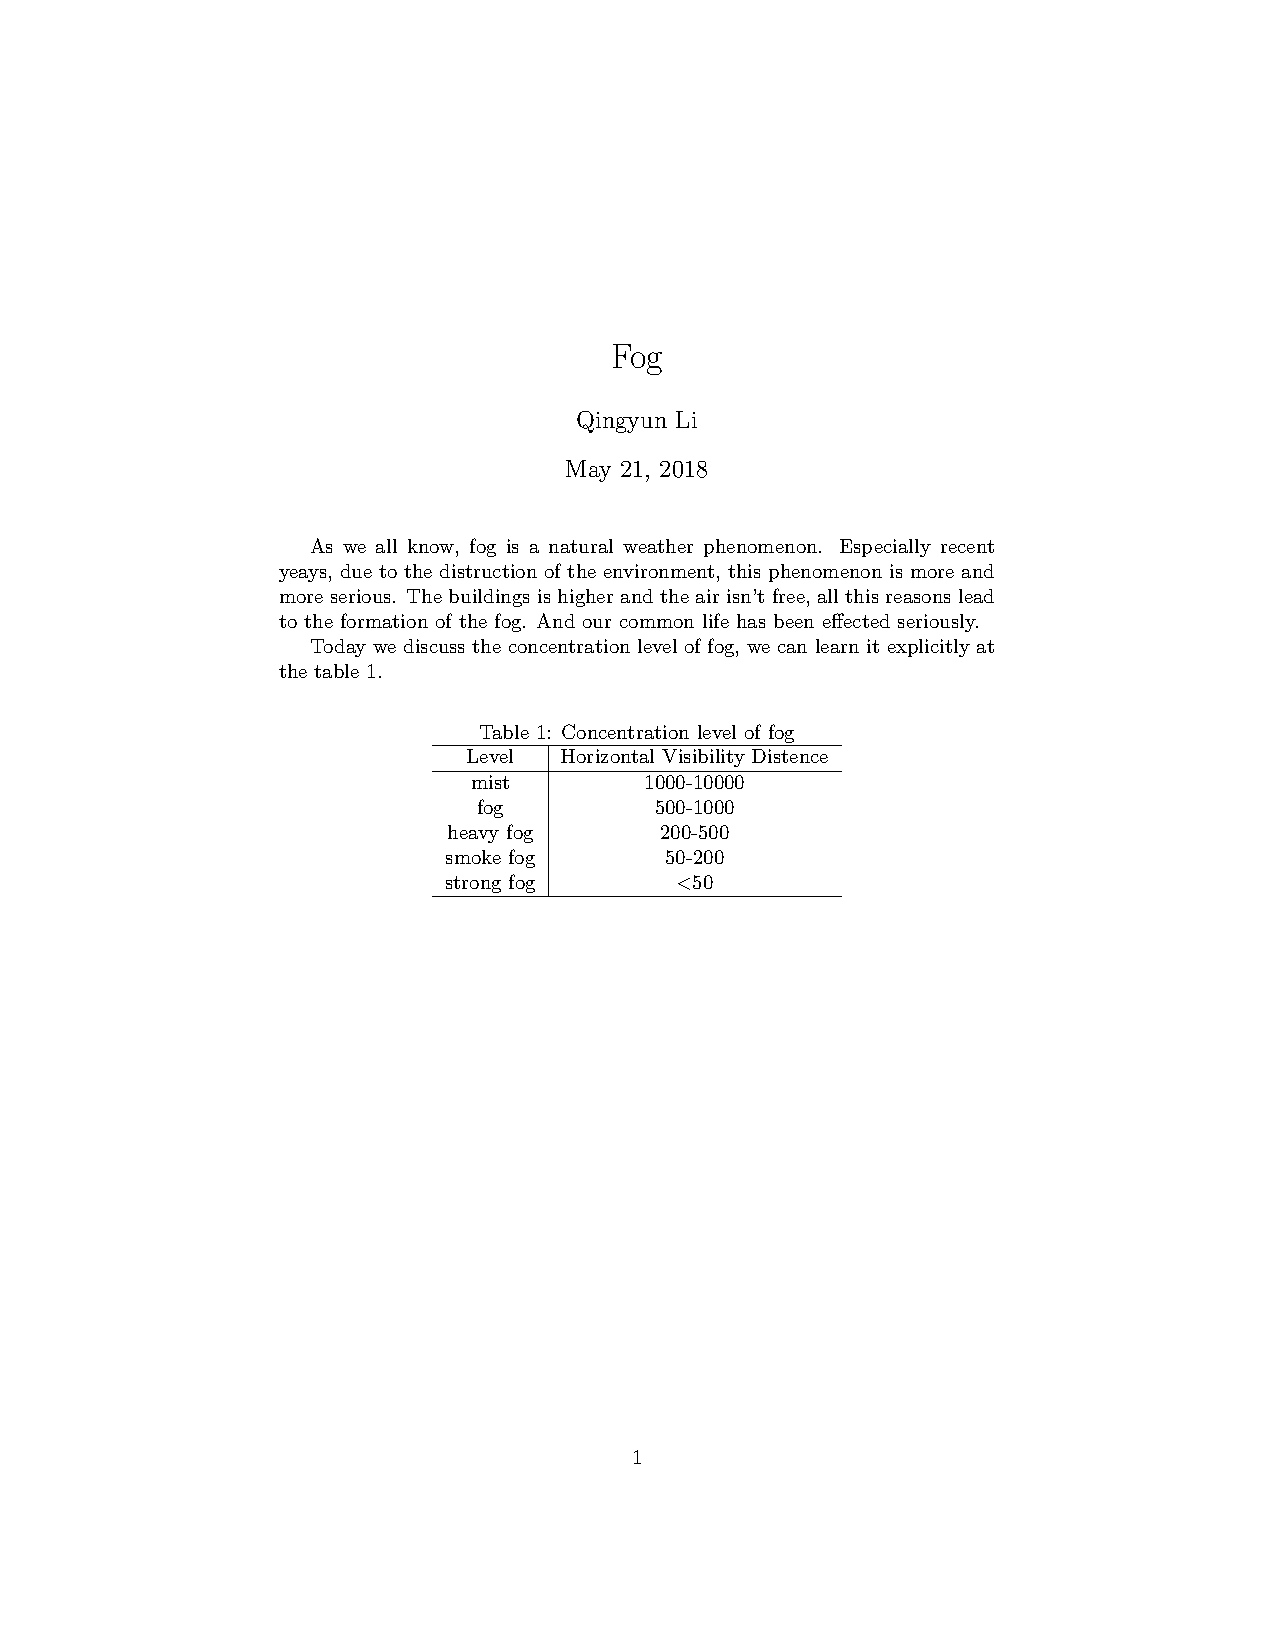
\includegraphics[width=0.4\textwidth]{Fog.jpeg} %\includegraphics[width=0.8\linewidth]{egfigure.eps}
\end{center}
   \caption{The difference of the fog and smog}
\label{difference}
\end{figure}

\section{Atmospheric light scattering model}
 \par The atmosphric light and the light reflected by the object itself combine with each other.And then, they enter the image acquisition device to form image.As is shown at Fig.~\ref{model1} So the suspended particles in the air and the incident light all effect the scattering effect of the atmosphere. When fog weather occurs, the amount of suspended particles increases. Therefore, in the process of image collection, the scattering and absorption of the radiated light is strengthened, and this resulted the color degradation and blurred details in the image.
\begin{figure}[htbp]
 \centering{}
\includegraphics[width=0.7\linewidth]{model1.jpeg}\\
 \caption{Atmospheric optical imaging model}
\label{model1}
\end{figure}

\section{Image degradation model}
 \par The degradation model is derived from the “Atmospheric light scattering model”, proposed by McCartney \emph{et al.}~\cite{Mccartney1976Optics}. A haze image formed as show in Fig.~\ref{model1} can be mathematically modeled as follows
\begin{equation}
I(x)=J(x)t(x)+A(1-t(x)) \label{eq1}
\end{equation}
\par This degradation model is consist of two parts, the first term of Eq.~\ref{eq1}, $J(x)t(x)$is the direct attenuation, and the second term of Eq.~\ref{eq1}, $A(1-t(x))$is the airlight.
\par The attenuation model means that the light reflection from the surface of the object encounters the sudpended particles and scatters, and part of the light deviates from the original direction, therefore, the incident light attenuates. This degree of attenuation is changes following the distance between the receiving device and the object. As the distance increases, the attenuation decays exponentially. The physical model is shown as Fig.~\ref{model2}.
\begin{figure}[htbp]
 \centering{}
\includegraphics[width=0.7\linewidth]{model2.jpg}\\
 \caption{The attenuation model}
\label{model2}
\end{figure}
\par The reflected light of the scene spots will attenuates because of the suspended particles, and at the same time, the sunlight and the reflected light of the ground will also scatter with the particles. This lead to the some of these light enters the receiving device and participates in imaging. These light called airlight. The physical model is shown as Fig.~\ref{model3}.  
\begin{figure}[htbp]
 \centering{}
\includegraphics[width=0.7\linewidth]{model3.jpg}\\
 \caption{Airlight}
\label{model3}
\end{figure} 

\section{Haze removal using dark channel prior}
\subsection{Dark channel prior}
\par DCP-dark channel prior. It was proposed by He \emph {et al.}~\cite{He2009Single} after they dealt with about 5000 outdoor free-haze images. They find that some pixels have a low intensity in at least one color channel, except for the sky region. And from 5000 dark channels of outdoor haze-free images, it was demonstrated that about 75 percent of the pixels in the dark channels have zero values and 90 percent of the pixels have values below 35. In conclusion, the approximation to zero for the pixel value of the dark channel is called DCP. We can see it at Fig.~\ref{dark1}.
 \begin{figure}[htbp]
 \centering{}
 \subfloat[]{\begin{minipage}{0.5\linewidth}
\includegraphics[width=0.9\linewidth]{cui.jpg}\\
 \end{minipage}}
 \hfill
\subfloat[]{\begin{minipage}{0.5\linewidth}
\includegraphics[width=0.9\linewidth]{cuidark.png}\\
\end{minipage}}
 \caption{(a) haze-free outdoor image, (b) dark channel}
\label{dark1}
\end{figure} 
\subsection{Patchsize}
 \par A key parameter in the algorithm is the patch size. On one hand, the dark channel prior becomes better for a larger patch size because the probability that a patch contains a dark pixel is increased. So the larger the patch size, the darker the dark channel. And in fact, we can use a larger patch to exclude false textures from the dark channel. As is shown at Fig.~\ref{dark2}.
 
\begin{figure}[htbp]
 \subfloat[]{\begin{minipage}{0.25\linewidth}
\includegraphics[width=0.9\linewidth]{forest.jpg}\\
 \end{minipage}}
\subfloat[]{\begin{minipage}{0.25\linewidth}
\includegraphics[width=0.9\linewidth]{dark3_3.png}\\
\end{minipage}}
 \subfloat[]{\begin{minipage}{0.25\linewidth}
\includegraphics[width=0.9\linewidth]{dark12_12.png}\\
 \end{minipage}}
\subfloat[]{\begin{minipage}{0.25\linewidth}
\includegraphics[width=0.9\linewidth]{dark15_15.png}\\
\end{minipage}}
 \caption{Dark channel of various patch size. (a) haze image. Dark channel with the patch size of (b) 3$\times$3, (c) 12$\times$12, (d) 15$\times$15}
\label{dark2}
\end{figure}

\subsection{Transmission map}
\par Due to this doscovery, the transmssion map $\tilde{t}(x) $ is obtained from the DCP accordding to the equation:
\begin{equation}
\tilde{t}(x)=1-\min\limits_{y\in\Omega(x)}(\min\limits_{c}\frac{I^{c}(y)}{A^c})
\end{equation}
\par However, in fact, the pixel value of dark channel, $J^{dark}(x)$, is not equivalent to zero completely. So, in order to make the image looked natural, we need to retain a small amount of haze by using a constant $\omega$ (0< $\omega$ <1):\begin{equation}
\tilde{t}(x)=1-\omega \min\limits_{y\in\Omega(x)}(\min\limits_{c}\frac{I^{c}(y)}{A^c})
\end{equation}
And inadvertently, we compensate for the under-estimation of $\tilde{t}(x)$ by multiplying $\omega$. When $\omega$ = 0.95, the transmission map is shown as Fig.~\ref{trans}.
 \begin{figure}[htbp]
 \centering{}
 \subfloat[]{\begin{minipage}{0.5\linewidth}
\includegraphics[width=0.9\linewidth]{cones.jpg}\\
 \end{minipage}}
 \hfill
\subfloat[]{\begin{minipage}{0.5\linewidth}
\includegraphics[width=0.9\linewidth]{trans3_3.png}\\
\end{minipage}}
 \caption{(a) haze image, (b) transmissinon map (3$\times$3)}
\label{trans}
\end{figure} 

 \bibliographystyle{ieee}
 \bibliography{single}
\end{document}
